\documentclass[ignorenonframetext,]{beamer}
\setbeamertemplate{caption}[numbered]
\setbeamertemplate{caption label separator}{: }
\setbeamercolor{caption name}{fg=normal text.fg}
\beamertemplatenavigationsymbolsempty
\usepackage{lmodern}
\usepackage{amssymb,amsmath}
\usepackage{ifxetex,ifluatex}
\usepackage{fixltx2e} % provides \textsubscript
\ifnum 0\ifxetex 1\fi\ifluatex 1\fi=0 % if pdftex
\usepackage[T1]{fontenc}
\usepackage[utf8]{inputenc}
\else % if luatex or xelatex
\ifxetex
\usepackage{mathspec}
\else
\usepackage{fontspec}
\fi
\defaultfontfeatures{Ligatures=TeX,Scale=MatchLowercase}
\fi
\usetheme{AnnArbor}
\usecolortheme{dolphin}
\usefonttheme{professionalfonts}
% use upquote if available, for straight quotes in verbatim environments
\IfFileExists{upquote.sty}{\usepackage{upquote}}{}
% use microtype if available
\IfFileExists{microtype.sty}{%
\usepackage{microtype}
\UseMicrotypeSet[protrusion]{basicmath} % disable protrusion for tt fonts
}{}
\newif\ifbibliography
\usepackage{longtable,booktabs}
\usepackage{caption}
% These lines are needed to make table captions work with longtable:
\makeatletter
\def\fnum@table{\tablename~\thetable}
\makeatother

% Prevent slide breaks in the middle of a paragraph:
\widowpenalties 1 10000
\raggedbottom

\AtBeginPart{
\let\insertpartnumber\relax
\let\partname\relax
\frame{\partpage}
}
\AtBeginSection{
\ifbibliography
\else
\let\insertsectionnumber\relax
\let\sectionname\relax
\frame{\sectionpage}
\fi
}
\AtBeginSubsection{
\let\insertsubsectionnumber\relax
\let\subsectionname\relax
\frame{\subsectionpage}
}

\setlength{\parindent}{0pt}
\setlength{\parskip}{6pt plus 2pt minus 1pt}
\setlength{\emergencystretch}{3em}  % prevent overfull lines
\providecommand{\tightlist}{%
\setlength{\itemsep}{0pt}\setlength{\parskip}{0pt}}
\setcounter{secnumdepth}{0}


% \pgfdeclareimage[width=1cm]{logo}{../Figures/antsCollaborators2.png}
%\logo{\pgfuseimage{logo}}

\institute{UCI}
\definecolor{links}{RGB}{42, 27, 129}
\definecolor{mypink2}{RGB}{219, 48, 122}
%\hypersetup{colorlinks,linkcolor=links,urlcolor=mypink2}
\usefonttheme{professionalfonts}

% \setbeamerfont{note page}{family*=pplx,size=\footnotesize} % Palatino for notes

\setbeamerfont{subtitle}{size=\small}

\definecolor{uciblue}{RGB}{0,100,164}
\definecolor{ucilibraryorange}{RGB}{255,210,0}
\definecolor{ucicream}{RGB}{241,229,199}
\definecolor{ucilightblue}{RGB}{163,220,230}

\setbeamercolor{block body}{bg=green,fg=green}
\setbeamercolor{block body alerted}{bg=green,fg=green}
\setbeamercolor{block body example}{bg=green,fg=green}

\setbeamercolor{caption name}{fg=uciblue}

\setbeamercolor{headline}{fg=ucicream,bg=ucicream}
\setbeamercolor{section}{fg=ucilibraryorange,bg=uciblue}
\setbeamercolor{frametitle}{fg=ucilibraryorange,bg=uciblue}
\setbeamercolor{palette primary}{bg=ucilibraryorange,fg=uciblue}
\setbeamercolor{palette secondary}{bg=uciblue,fg=uciblue}
\setbeamercolor{palette tertiary}{bg=ucilibraryorange,fg=uciblue}
\setbeamercolor{palette quarternary}{fg=ucilibraryorange,bg=uciblue}
\setbeamercolor{palette sidebar primary}{bg=ucilibraryorange,fg=uciblue}
\setbeamercolor{palette sidebar secondary}{fg=uciblue,bg=uciblue}
\setbeamercolor{palette sidebar tertiary}{fg=ucilibraryorange,bg=uciblue}
\setbeamercolor{palette sidebar quarternary}{fg=ucilibraryorange,bg=uciblue}
\setbeamercolor{structure}{bg=uciblue}



\useinnertheme{rectangles}

\titlegraphic{\vspace{-7.5mm}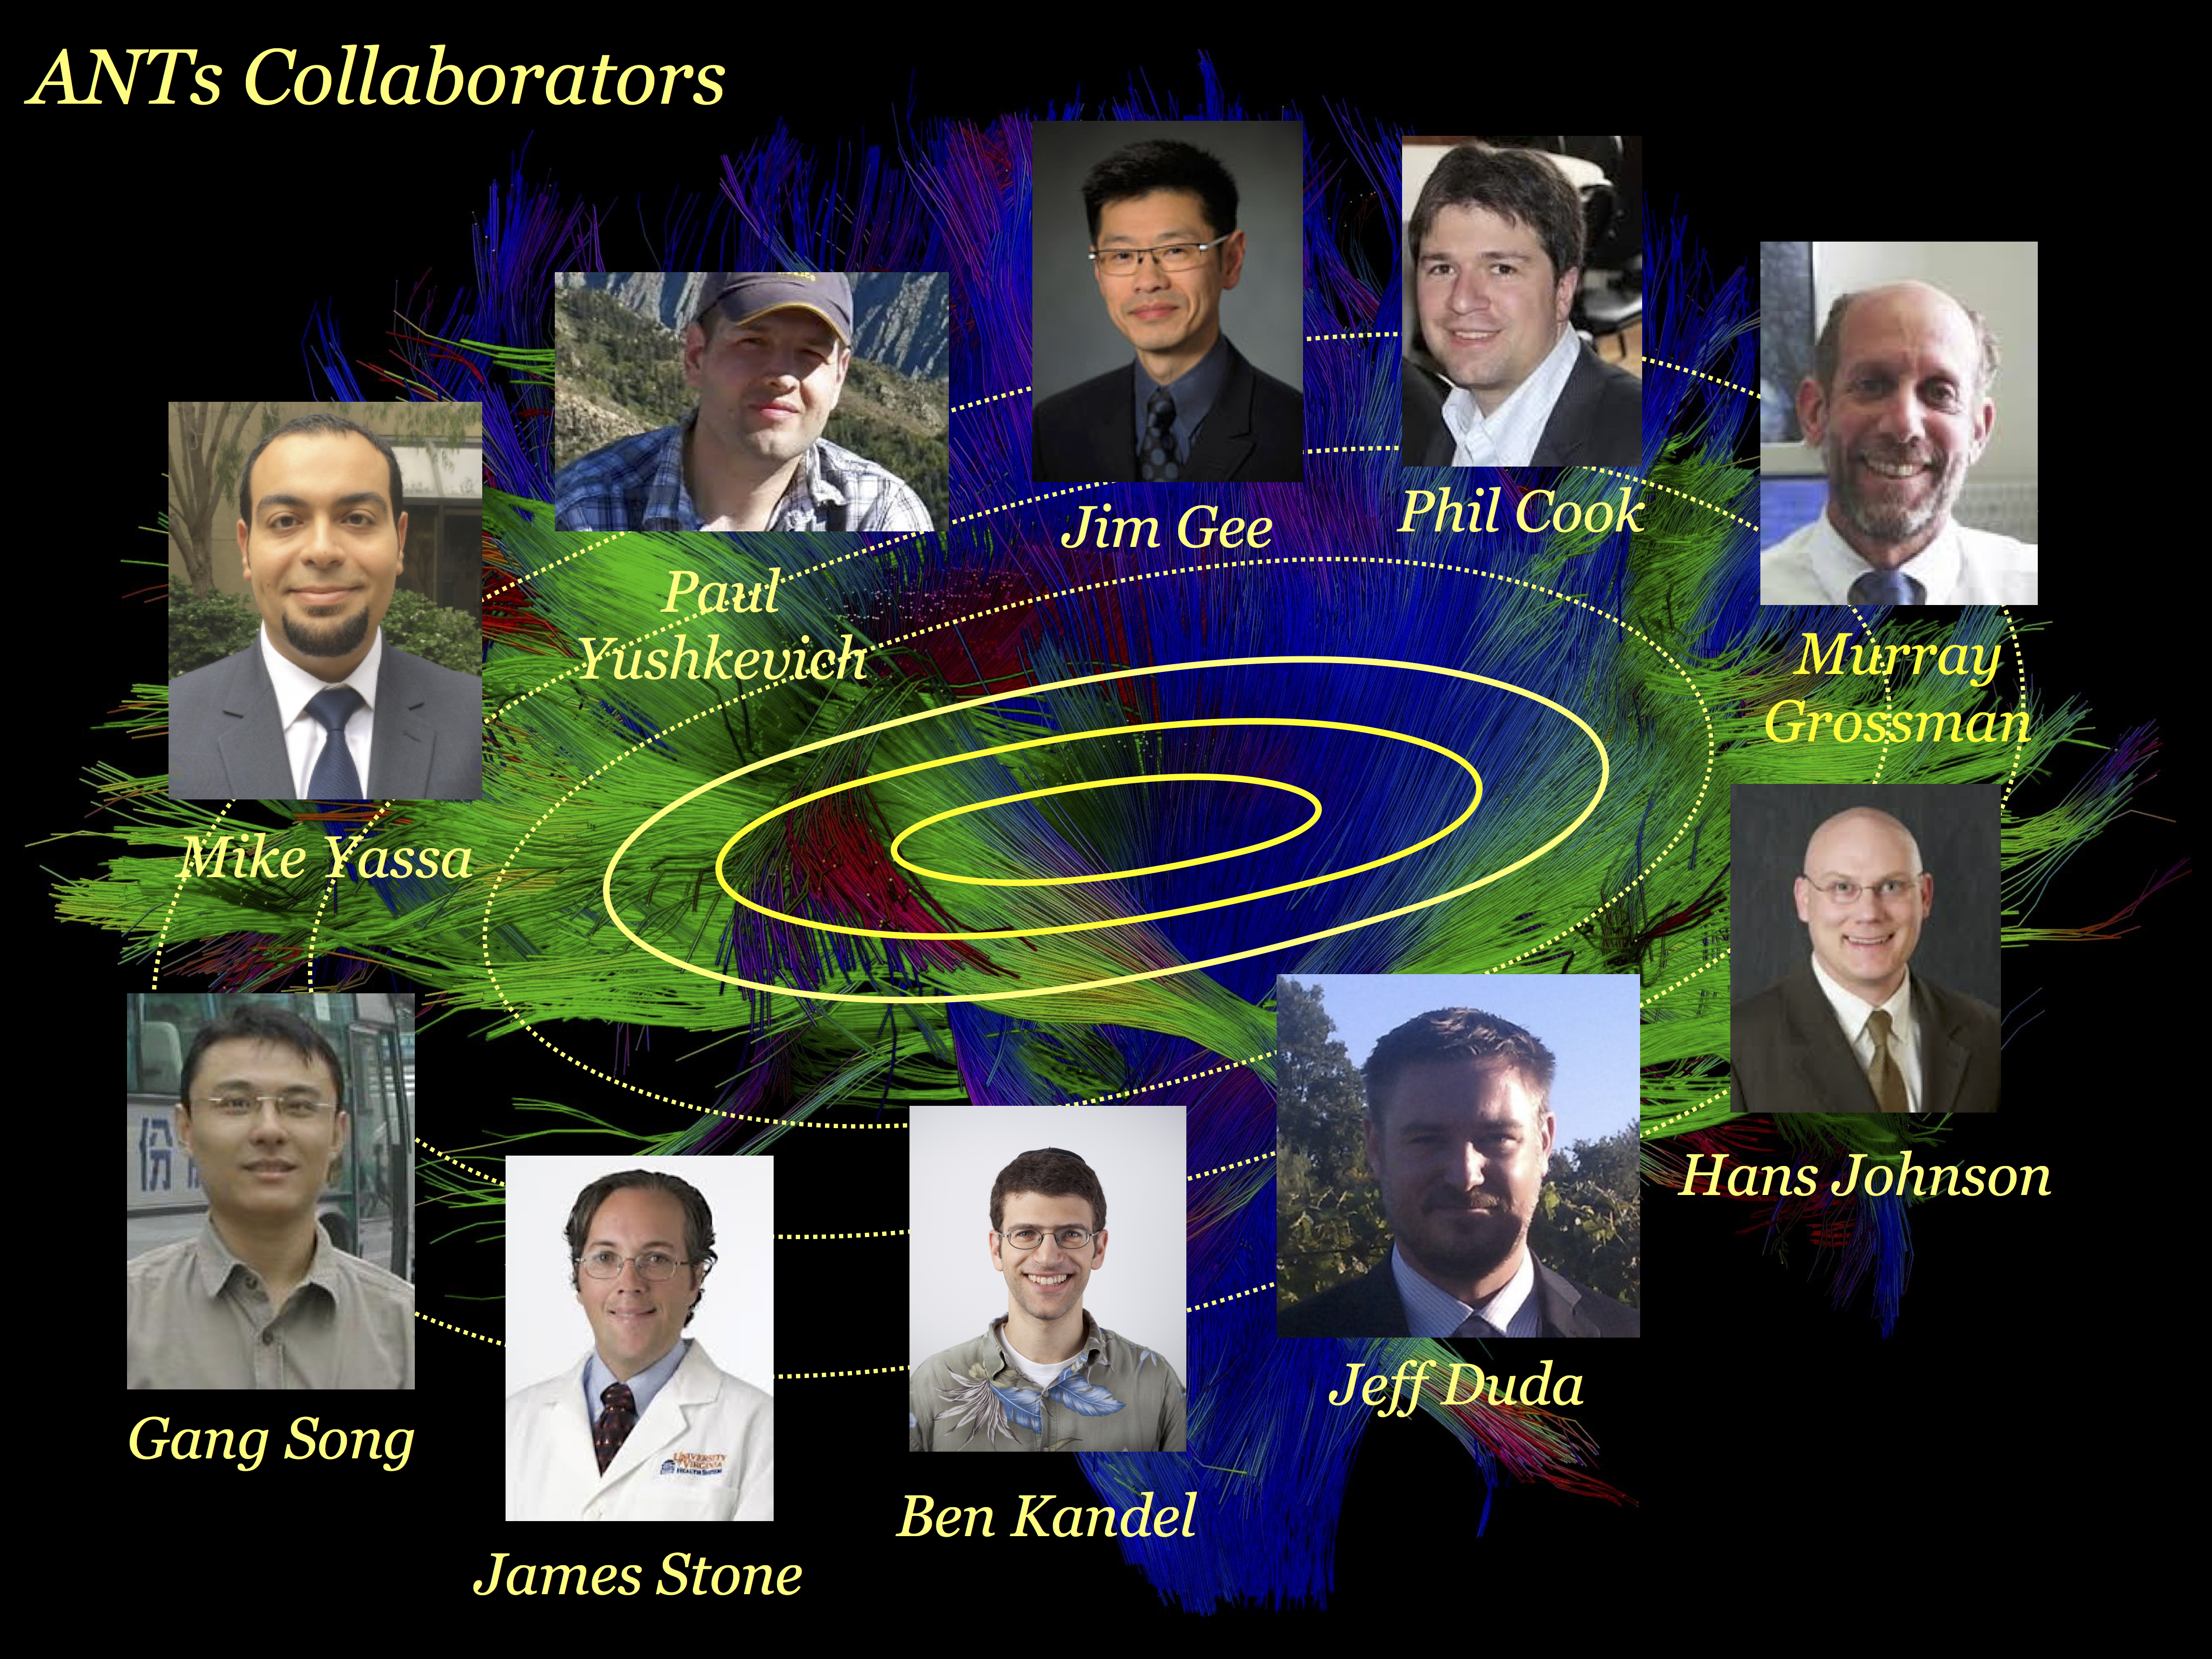
\includegraphics[width=0.45\paperwidth]{../Figures/antsCollaborators2.png}}

\title{ASHS revisited --- can we do better?}
\author{Nick Tustison and Mike Yassa}
\date{}

\begin{document}
\frame{\titlepage}

\section{Motivation}\label{motivation}

\begin{frame}{ASHS overview}

\centering
\includegraphics[width=0.85 \textwidth]{../Figures/ashs.png}

\end{frame}

\section{Joint Label Fusion}\label{joint-label-fusion}

\begin{frame}[fragile]{Modifications}

\begin{itemize}
\tightlist
\item
  Registration

  \begin{itemize}
  \tightlist
  \item
    \texttt{ANTS} \(\rightarrow\) \texttt{antsRegistration}
  \item
    B-spline SyN (``\texttt{-t\ BSplineSyN{[}...{]}}'')
  \item
    \texttt{WarpImageMultiTransform} \(\rightarrow\)
    \texttt{antsApplyTransforms}
  \item
    generic label interpolation
    (``\texttt{-n\ GenericLabel{[}Linear{]}}'')
  \end{itemize}
\item
  \texttt{jointfusion} \(\rightarrow\) \texttt{antsJointFusion}

  \begin{itemize}
  \tightlist
  \item
    non-negative least squares option (vs.~SVD)
  \item
    multi-threaded
  \item
    memory issues
  \item
    joint intensity fusion
  \end{itemize}
\end{itemize}

\end{frame}

\begin{frame}{Registration --- beyond original SyN}

\centering
\includegraphics[width=0.85 \textwidth]{../Figures/Frontiers_ITK.png}

\vspace{2mm}

\centering
\includegraphics[width=0.85 \textwidth]{../Figures/Frontiers_BSplineSyN.png}

\end{frame}

\begin{frame}{T2 joint intensity fusion}

\centering
\includegraphics[width=0.85 \textwidth]{../Figures/jifNormalization.png}

\end{frame}

\begin{frame}{T2 joint intensity fusion sample results}

\centering
\includegraphics[width=0.85 \textwidth]{../Figures/jifResults.png}

\end{frame}

\section{Corrective learning}\label{corrective-learning}

\begin{frame}{Modifications}

\begin{itemize}
\tightlist
\item
  machine learning technique

  \begin{itemize}
  \tightlist
  \item
    AdaBoost (original ASHS)
  \item
    random forests
  \item
    extreme gradient boosting
  \end{itemize}
\item
  ANTsR implementation

  \begin{itemize}
  \tightlist
  \item
    open-source
  \item
    easy to
    \href{https://github.com/stnava/ANTsR/blob/master/R/segmentationRefinement.R\#L375-L413}{change}
    machine learning techniques
  \end{itemize}
\item
  prior knowledge

  \begin{itemize}
  \tightlist
  \item
    two classes (original ASHS)
  \item
    four classes
  \end{itemize}
\end{itemize}

\end{frame}

\begin{frame}{}

\centering
\includegraphics[width=0.85 \textwidth]{../Figures/machineLearningTechniques.png}

\end{frame}

\begin{frame}{ANTsR facilitates technique substitution}

\centering
\includegraphics[width=0.85 \textwidth]{../Figures/segRefinement.png}

\end{frame}

\begin{frame}{Incorporate additional prior knowledge}

\centering
\includegraphics[width=0.85 \textwidth]{../Figures/correctiveLearning001.png}

\end{frame}

\begin{frame}{Two-class AdaBoost}

\centering
\includegraphics[width=0.85 \textwidth]{../Figures/correctiveLearning002.png}

\end{frame}

\begin{frame}{Four-class random forest or extreme gradient boosting}

\centering
\includegraphics[width=0.85 \textwidth]{../Figures/correctiveLearning003.png}

\end{frame}

\section{Results}\label{results}

\begin{frame}{Summary}

\centering
\includegraphics[width=0.85 \textwidth]{../Figures/summaryResults.png}

\end{frame}

\begin{frame}{Data overview}

\begin{itemize}
\tightlist
\item
  Penn data

  \begin{itemize}
  \tightlist
  \item
    Yushkevich et al., Hum Brain Mapp. 2015 Jan; 36(1): 258--287.
  \item
    29 subjects
  \item
    10 labels per hemisphere (2 are discarded prior to analysis)
  \item
    hippocampal subfields and extrahippocampal cortical structures
    (ERC/PRC/PHC)
  \end{itemize}
\item
  UCI Data (``Stark Training Set'')

  \begin{itemize}
  \tightlist
  \item
    19 subjects
  \item
    3 labels per hemisphere
  \item
    ?
  \end{itemize}
\end{itemize}

\end{frame}

\begin{frame}{Penn data}

\centering
\includegraphics[width=1 \textwidth]{../Figures/pennResults.png}

\end{frame}

\begin{frame}{UCI data}

\centering
\includegraphics[width=1 \textwidth]{../Figures/uciResults.png}

\end{frame}

\begin{frame}{Penn data: JLF T1-only}

\begin{longtable}[c]{@{}lrrrrrrrrr@{}}
\toprule
& all & 1 & 2 & 3 & 4 & 8 & 9 & 11 & 12\tabularnewline
\midrule
\endhead
left & 0.61 & 0.65 & 0.08 & 0.70 & 0.33 & 0.53 & 0.61 & 0.48 &
0.58\tabularnewline
right & 0.56 & 0.62 & 0.10 & 0.67 & 0.32 & 0.53 & 0.58 & 0.42 &
0.51\tabularnewline
\bottomrule
\end{longtable}

\end{frame}

\begin{frame}{Penn data: Xgb Min T1-only}

\begin{longtable}[c]{@{}lrrrrrrrrr@{}}
\toprule
& all & 1 & 2 & 3 & 4 & 8 & 9 & 11 & 12\tabularnewline
\midrule
\endhead
left & 0.65 & 0.69 & 0.12 & 0.73 & 0.36 & 0.56 & 0.65 & 0.57 &
0.65\tabularnewline
right & 0.63 & 0.67 & 0.15 & 0.72 & 0.36 & 0.57 & 0.64 & 0.53 &
0.60\tabularnewline
\bottomrule
\end{longtable}

\end{frame}

\begin{frame}{UCI data: JLF T1-only}

\begin{longtable}[c]{@{}lrrrrrrr@{}}
\toprule
& all & 13 & 15 & 17 & 14 & 16 & 18\tabularnewline
\midrule
\endhead
left & 0.739 & 0.708 & 0.753 & 0.732 & NaN & NaN & NaN\tabularnewline
right & 0.738 & NaN & NaN & NaN & 0.705 & 0.752 & 0.735\tabularnewline
\bottomrule
\end{longtable}

\end{frame}

\begin{frame}{UCI data: Xgb Min T1-only}

\begin{longtable}[c]{@{}lrrrrrrr@{}}
\toprule
& all & 13 & 15 & 17 & 14 & 16 & 18\tabularnewline
\midrule
\endhead
left & 0.753 & 0.727 & 0.767 & 0.741 & NaN & NaN & NaN\tabularnewline
right & 0.747 & NaN & NaN & NaN & 0.716 & 0.762 & 0.74\tabularnewline
\bottomrule
\end{longtable}

\hypertarget{refs}{}

\end{frame}

\end{document}
